\subsubsection{Components of usability}
Based on Nielsen 2012 (https://medium.com/@iizzathisharah/the-five-usability-components-by-jakob-nielsen-detailed-insights-and-examples-90695af5ffb6)

\begin{itemize}
    \item learnability
    \item efficiency
    \item memorabiliy
    \item errors
    \item satisfaction
\end{itemize}

\newpage
\subsubsection{Usability testing}
\sloppy
Magpie has remedied the first challenge of fragmented information on amenities. We will now address the second challenge: making the access to this information easy, quick \& accessible.\\

\noindent The goal of the user evaluation is to gain feedback from real users, learn if Magpie works as expected and assess overall user interface. Our approach is as follows:
%user evaluation approach
\begin{enumerate}
    \item Round up users from the market research + seek out others
    \item Conduct online usability sessions to discuss Magpie, explore the features, gather feedback,
    \item Synthesize notes from sessions and summarize points to improve
    \item Iteratively implement/improve features
\end{enumerate}
We interviewed 11 users in total. They have been divided into the following categories: 6 general users, 3 targeted users, 1 UI/UX expert and 1 accessibility expert.\\
\emph{General users} are defined as those who use Magpie casually for personal interests.\\ \emph{Targeted users} are defined as those who use Magpie as a tool for their work.

\noindent Both controlled \& uncontrolled approaches were used for the sessions.\\
The controlled sessions were based around a strict list of tasks the user would complete and used metrics such as time taken, difficulty and task success rate.\\
The uncontrolled sessions let the users freely roam the application while we observed their behaviour interacting with each element and initiate discussion to obtain feedback on features to improve.\\

\noindent A table with a list of general tasks is used to quantitatively evaluate each feature the user interacted with. Metrics measured are task difficulty and task success rate. The list of general tasks increased as the test sessions went on because new features were being added iteratively.\\
The difficulty of the task is related to its status and how much time a user spent on it. The status of a task can either be "complete", "pass", or "fail" where:
\begin{itemize}
    \item "complete" is attributed when the user completes the task on their own
    \item "pass" is attributed when the user was able to complete the task but with our help
    \item "fail" is attributed when the user was not able to complete the task even with our help
\end{itemize}
Lastly, a short satisfaction survey is administered at the end of each session quantify user experience and provide a baseline for improvements. User behaviour is also observed during the session to complement these quantitative metrics.\\
%figure for satisfaction survey
\begin{figure}
    \centering
    \fbox{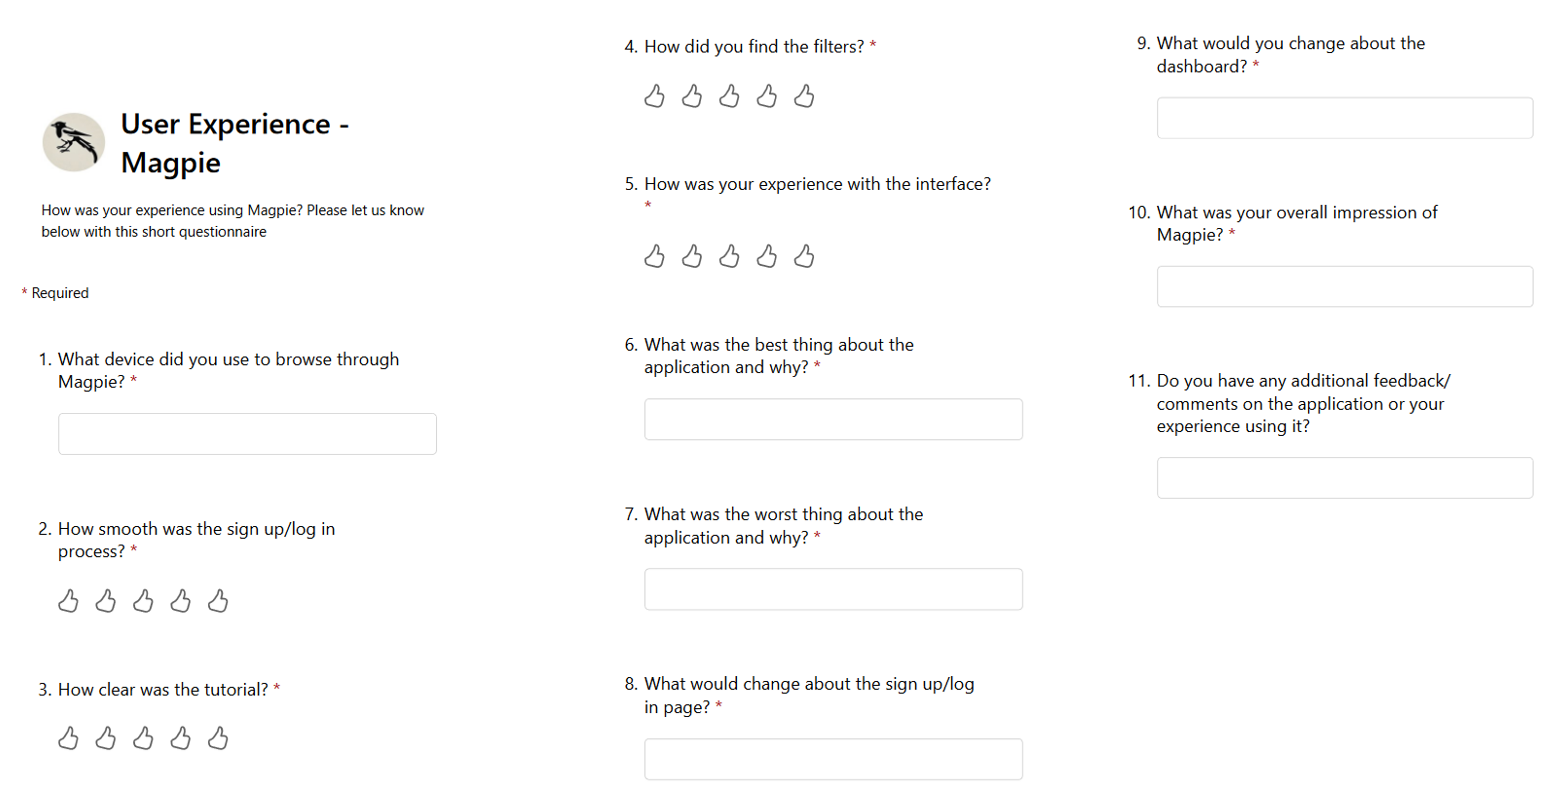
\includegraphics[width=0.8\textwidth]{images/user-satisfaction-survey.png}}
    \caption{User Evaluation - Satisfaction survey questions}
\end{figure}

\newpage
\subsubsection{User 1 - Brendan}
Brendan is a professor with technological background. They are considered a casual user.\\\\
This was an uncontrolled test session where Brendan tested each feature of Magpie to find faults, system failures and bugs.\\\\
\textbf{Main takeaways from Brendan's session: }Magpie has potential for use by certain types of users but needs a lot more functionality. Here is a breakdown of the feedback:
\begin{itemize}
    \item \textbf{Log in/Sign up: }why is a username required? Username should be the email. And email verification is a must!
    \item \textbf{Tutorial: }content of step 2 needs to be reworked, explain radius of what. Also, the positioning of certain elements is off in Firefox browser. For step 4, content wording change “dozen” for something else especially if you're planning on adding more amenity data. The step 5 should point to the map, investigate the bug.
    \item \textbf{Dashboard: }you should implement a button to clear the market and all the points from the map, right now the user has to reload. Perhaps think of leaving the count of toggled off amenities, it would depend on the use case. Maybe implement a quick reset button for  selected amenities. Compress list of amenities to avoid scrolling (window size issue in Firefox browser)
    \item \textbf{Map: } you need to add plus and minus buttons to zoom in and out of the map. Can I have more information from the amenity icons by clicking on them? Perhaps a marked up image that detects this space (google street view), information on the spot (private, free, carpark). Also, make the selected icons more visually striking, a little hover maybe
    \item \textbf{Technical: }when clicking on map, there is a slight offset between where the marker appears and where the user clicked; implement something to avoid mis-clicking and loosing original marker position; Icons move when you toggle on and off certain amenities
    \item \textbf{Misc: }why are we requesting location? For the marker data (maybe we should let the user know this is where they are on the map?); need a landing page to present magpie; is the version prototype logo useful? Maybe for dev; show more information and the ml images we worked on (personal preference); reiterates we should put the ml forward (maybe on the about us)
\end{itemize}
\textbf{Overall: }the interface is nice, but you might want to focus on producing a much more data-driven approach for the interface if you want to attract those kinds of users. Brendan was very tempted to click on the amenity icons of the map to find out more information.\\\\
\textbf{Score from survey: }
%brendan survey score
\begin{figure}
    \centering
    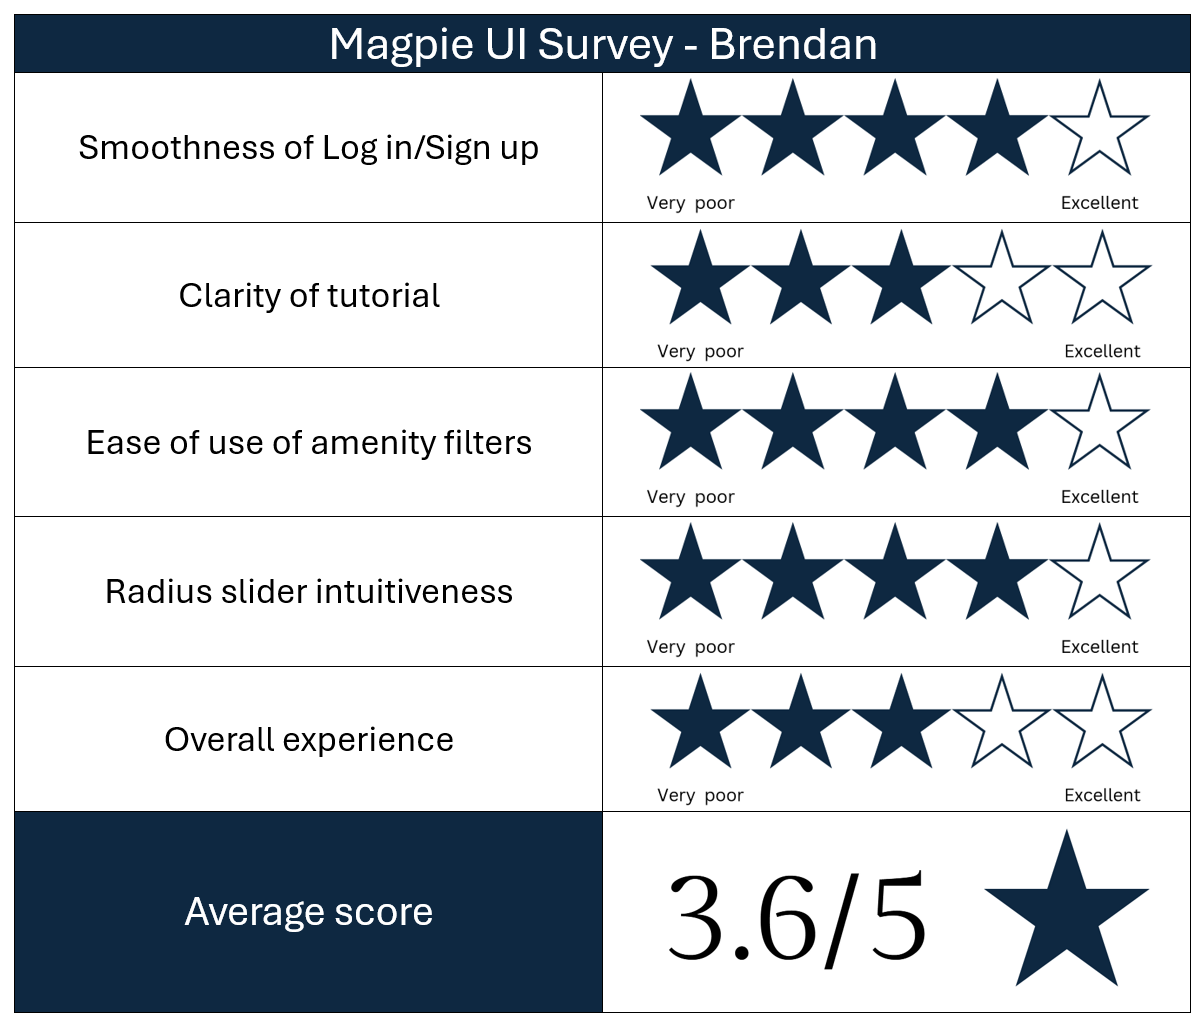
\includegraphics[width=0.8\textwidth]{images/survey-brendan.png}
    \caption{User Evaluation - UI Score Brendan}
\end{figure}

\newpage
\subsubsection{User 2 - Anonymous (Maira)}
This user has a background in technology at the doctorate level.\\
This session was mostly uncontrolled, they browsed the application, tested the features and discussed their thoughts with us.\\\\
\textbf{Main takeaways from the session: } this user really enjoyed the presentation of information on the application, they found the amenities easy to understand and recognizable in the radius of the map.\\\\
They tried to interact with the locked elements of the tutorial, and really enjoyed the confetti at the end of it. Also, before placing a marker on the map because when they accepted location tracking, their own marker appeared.\\\\
To make more improvements, they suggested the following:
\begin{itemize}
    \item \textbf{More features: }They feel like a search bar would help in the quest for information in specific location visually unknown to the user. They also though the points would appear automatically on the map but instead she had to place her own marker. Perhaps there is an issue with onboarding not being retained.
    \item \textbf{Dashboard \& Map: }There is an icon, the water fountain one that is neon blue, therefore blends into the white background of the dashboard and in the map; probably needs to be changed. Also, more data for example on transportation would be a big plus.
    \item \textbf{Misc: } If you want to appeal to more general users, adding more features like location sharing, integrating social interactions and make it mobile responsive would be the way to go. Also, a higher level of information.
\end{itemize}
\textbf{Overall: }it is a very good application, a very interesting idea to gather all this information in one place.\\\\
\textbf{Score from survey: }
%maira survey score
\begin{figure}
    \centering
    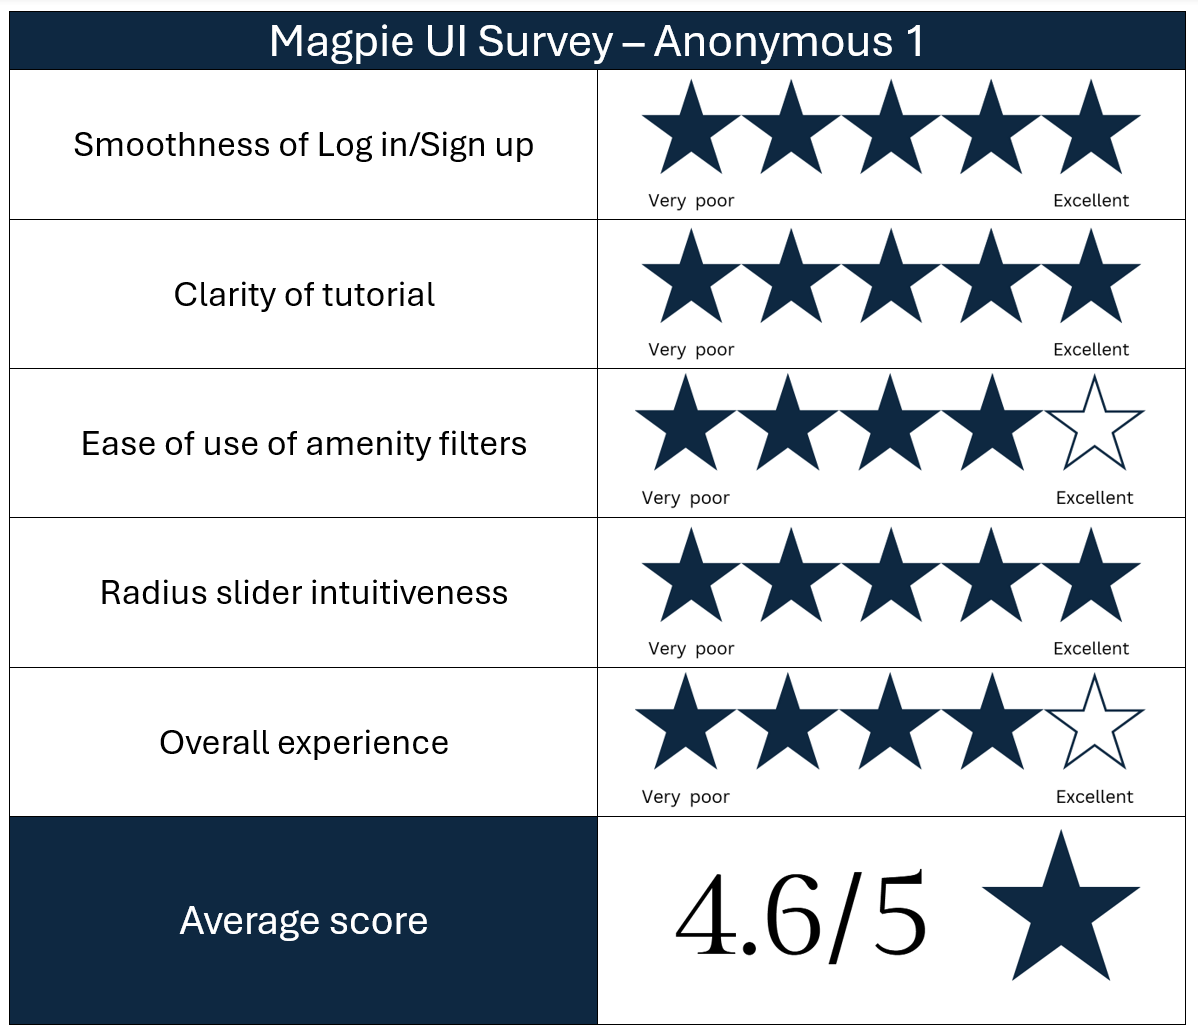
\includegraphics[width=0.8\textwidth]{images/survey-maira.png}
    \caption{User Evaluation - UI Score Anonymous 1}
\end{figure}

\newpage
\subsubsection{User 3 - Paul}
Our second controlled session was with Paul, a student in technological undergraduate degree. They are classified as a general user, not one we have identified as our target. They left their contact email in the market research survey.\\
We initially wanted this to be a controlled test session by giving him specific tasks, but found that challenging as he intuitively went on to explore the application on his own.
%table of Paul's general tasks
\begin{table}[h!]
    \centering
    \caption{Usability testing Tasks - Paul}
    \begin{tabular}{|p{0.4\textwidth}|p{0.1\textwidth}|p{0.1\textwidth}|p{0.1\textwidth}|p{0.1\textwidth}|}
        \hline
        \textbf{Task}                                 & \textbf{Status} & \textbf{Time taken} & \textbf{Difficulty} & \textbf{Errors}    \\
        \hline
        Load Magpie application                       & Complete        & 20s                 & 1                   & N/A                \\
        \hline
        Sign up                                       & Complete        & 42s                 & 1                   & N/A                \\
        \hline
        Complete tutorial                             & Complete        & 60s                 & 1                   & N/A                \\
        \hline
        Place cursor on map and adjust radius to 250m & Fail            & Skipped             & Skipped             & Skipped            \\
        \hline
        Zoom in to road name level                    & Complete        & 5s                  & 1                   & N/A                \\
        \hline
        Place cursor on another area                  & Complete        & 5s                  & 1                   & N/A                \\
        \hline
        Zoom out to see full radius                   & Fail            & Skipped             & Skipped             & Skipped            \\
        \hline
        Filter to only view "Parking meter" data      & Pass            & 120s                & 3                   & Required help      \\
        \hline
        Filter to toggle off all amenities            & Pass            & 37s                 & 3                   & Required help      \\
        \hline
        Go through tutorial and exit at Step 3        & Pass            & 30s                 & 3                   & Couldn't find icon \\
        \hline
        Log out                                       & Complete        & 20s                 & 2                   & N/A                \\
        \hline
    \end{tabular}
\end{table}
\textbf{Main takeaways from Paul's session: }the map display and the amenity data displayed is "excellent", they would find it useful for local areas of the city. One aspect they advise we improve on is to make the choice of amenities more intuitive. This is further supported by his behaviour trying to click on the icon and subsequent amenity title on the dashboard to toggle it on and off, as well as the difficulties he encountered as shown in the general task table.\\
Another point to improve on is to make the profile and tutorial icons more visible, demonstrated by the time it took him to find them and complete the general tasks.\\\\
\textbf{Score from survey: }
%paul survey score
\begin{figure}
    \centering
    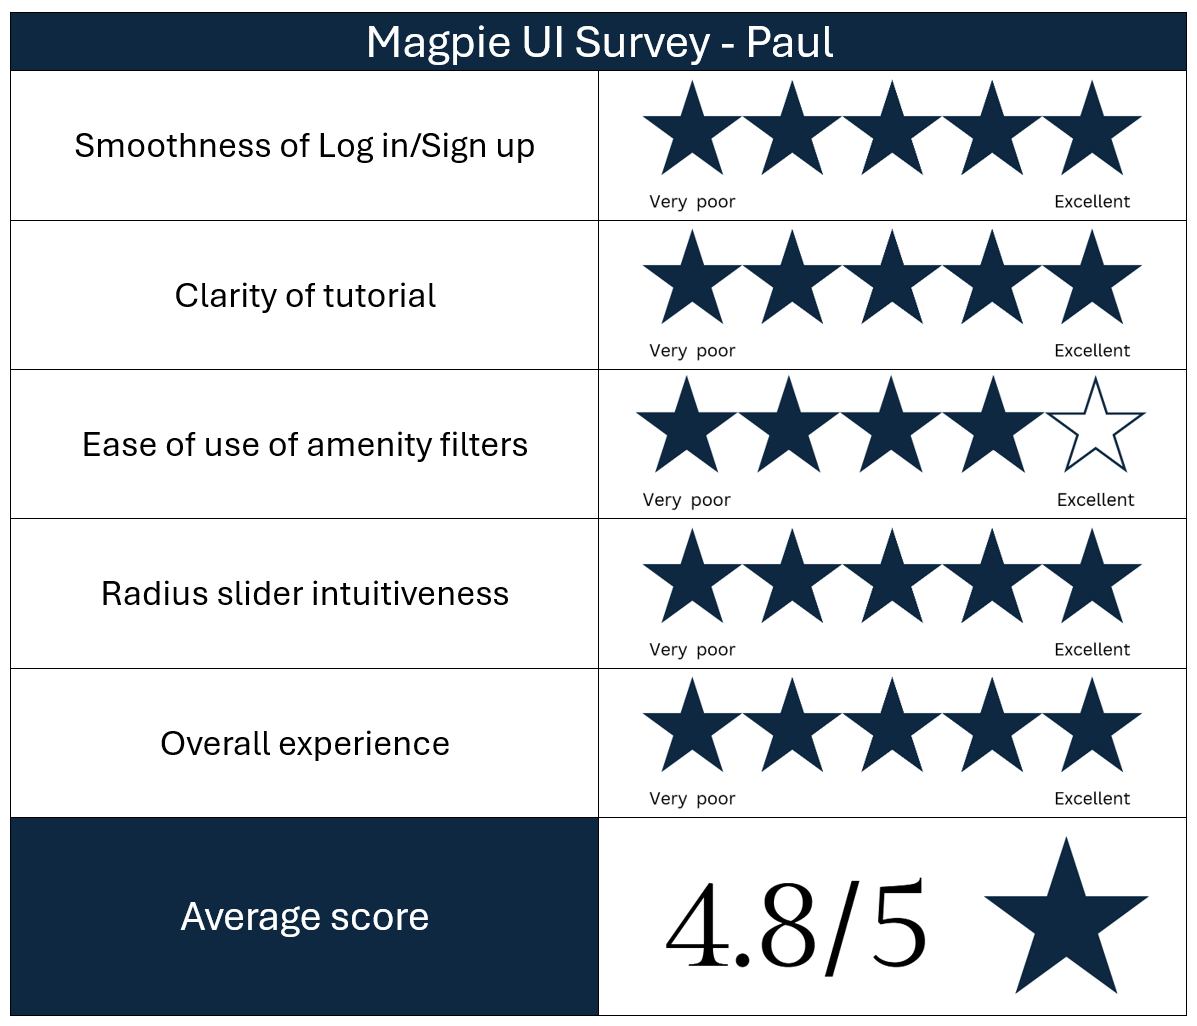
\includegraphics[width=0.8\textwidth]{images/survey-paul.png}
    \caption{User Evaluation - UI Score Paul}
\end{figure}

\newpage
\subsubsection{User 4 - Livia}
Our third controlled session was with Livia, another student in a technological undergraduate degree. They are also identified as a casual user who also left their contact in the market research survey.\\\\
This session also started out as a controlled test with a defined set of tasks, but just like Paul, Livia went on to explore the application skipping the tasks.\\\\
%table of Livias's general tasks
\begin{table}[h!]
    \centering
    \caption{Usability testing Tasks - Livia}
    \begin{tabular}{|p{0.4\textwidth}|p{0.1\textwidth}|p{0.1\textwidth}|p{0.1\textwidth}|p{0.1\textwidth}|}
        \hline
        \textbf{Task}                                 & \textbf{Status} & \textbf{Time taken} & \textbf{Difficulty} & \textbf{Errors} \\
        \hline
        Load Magpie application                       & Complete        & 5s                  & 1                   & N/A             \\
        \hline
        Sign up                                       & Complete        & 16s                 & 1                   & N/A             \\
        \hline
        Complete tutorial                             & Complete        & 44s                 & 1                   & N/A             \\
        \hline
        Place cursor on map and adjust radius to 250m & Complete        & 6s                  & 1                   & N/A             \\
        \hline
        Zoom in to road name level                    & Complete        & 8s                  & 1                   & N/A             \\
        \hline
        Place cursor on another area                  & Fail            & Skipped             & Skipped             & Skipped         \\
        \hline
        Zoom out to see full radius                   & Fail            & Skipped             & Skipped             & Skipped         \\
        \hline
        Filter to only view "Parking meter" data      & Fail            & Skipped             & Skipped             & Skipped         \\
        \hline
        Filter to toggle off all amenities            & Complete        & 18s                 & 1                   & N/A             \\
        \hline
        Go through tutorial and exit at Step 3        & Complete        & 24s                 & 2                   & N/A             \\
        \hline
        Log out                                       & Complete        & 20s                 & 2                   & N/A             \\
        \hline
    \end{tabular}
\end{table}
\textbf{Main takeaways from Livia's session: }very interesting project, useful and great; overall a very clear website. Biggest point of discontent for Livia was the tutorial, they let us know they has dyslexia and the tutorial could've been worded more effectively to cater to them and others with learning/visual impediments. In addition, they tried to interact with the locked elements during the tutorial, suggesting intuition to put in practice what they are reading to validate the information absorbed.\\\\
They also suggested adding more amenities such as public transports stops, scooter stands and student hubs. They liked how it was easier to understand the information visually compared to Google maps or Apple maps.\\\\
\textbf{Score from survey: }
%livia survey score
\begin{figure}
    \centering
    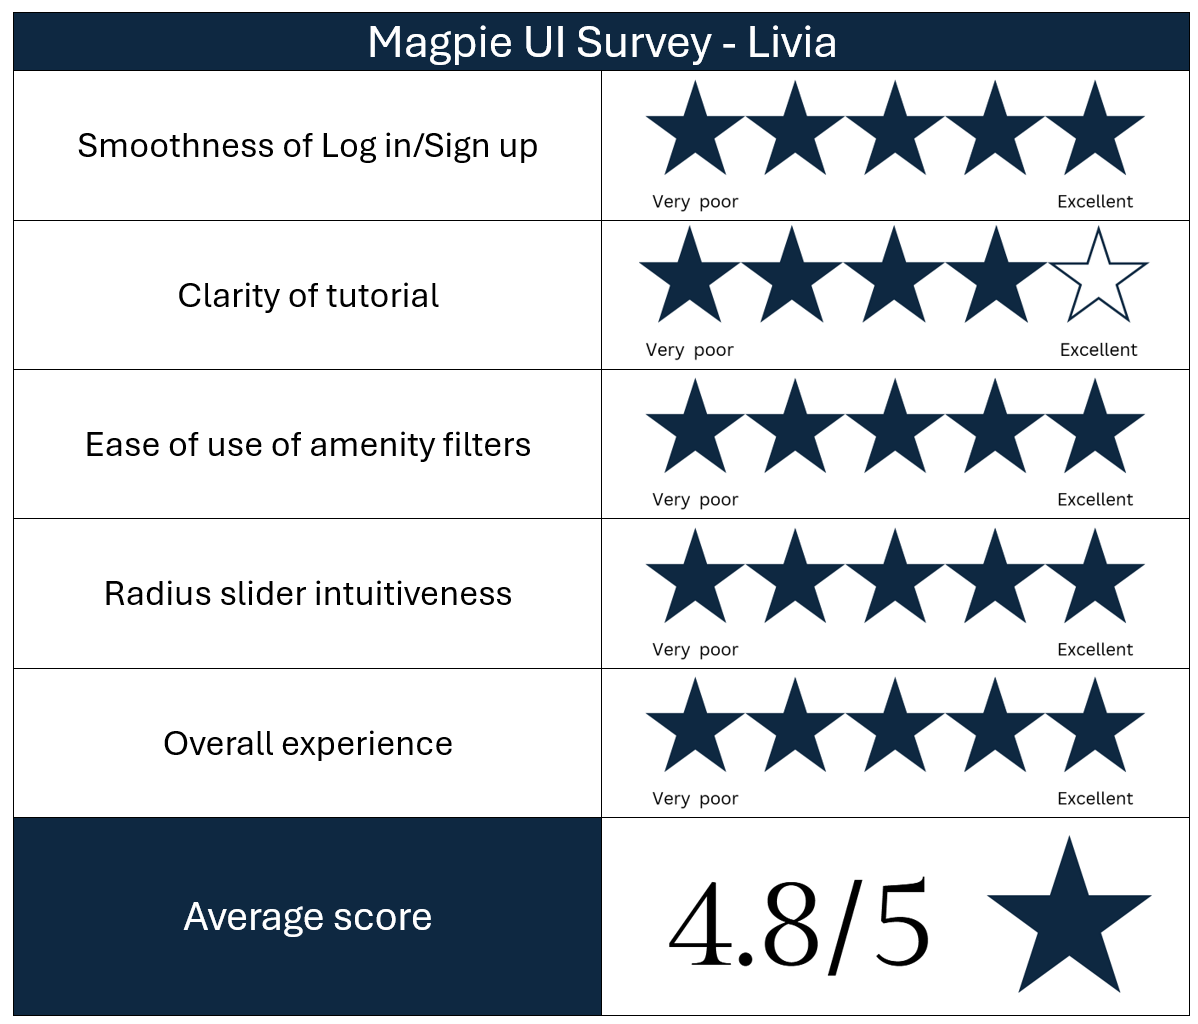
\includegraphics[width=0.8\textwidth]{images/survey-livia.png}
    \caption{User Evaluation - UI Score Livia}
\end{figure}

\newpage
\subsubsection{User 5 - Ben}
Our next test session was with Ben, another student in a technological post-graduate degree. They are also identified as a casual user who also left their contact in the market research survey.\\\\
Starting this session, we took a more uncontrolled approach and let the users free roam the application without giving them specific tasks to complete. We guided them in the beginning and initiated certain discussions but overall let the users take the reign and think aloud during their exploration process.\\\\
%table of Ben's general tasks
\begin{table}[h!]
    \centering
    \caption{Usability testing Tasks - Ben}
    \begin{tabular}{|p{0.4\textwidth}|p{0.1\textwidth}|p{0.1\textwidth}|p{0.1\textwidth}|p{0.1\textwidth}|}
        \hline
        \textbf{Task}                 & \textbf{Status} & \textbf{Difficulty} & \textbf{Errors} \\
        \hline
        Load Magpie application       & Complete        & 1                   & N/A             \\
        \hline
        Sign up                       & Complete        & 1                   & N/A             \\
        \hline
        Log in                        & Complete        & 1                   & N/A             \\
        \hline
        Complete tutorial             & Complete        & 1                   & N/A             \\
        \hline
        Place cursor on map           & Complete        & 1                   & N/A             \\
        \hline
        Zoom in and out               & Complete        & 1                   & N/A             \\
        \hline
        Hold map and navigate         & Complete        & 1                   & N/A             \\
        \hline
        Adjust radius big/small       & Complete        & 1                   & N/A             \\
        \hline
        Clear marker \& radius        & Skipped         & Skipped             & Skipped         \\
        \hline
        Deselect all amenities        & Complete        & 1                   & N/A             \\
        \hline
        Select one or more amenities  & Complete        & 1                   & N/A             \\
        \hline
        Find tutorial and exit midway & Skipped         & Skipped             & Skipped         \\
        \hline
        Log out                       & Complete        & 1                   & N/A             \\
        \hline
    \end{tabular}
\end{table}
\textbf{Main takeaways from Ben's session: }the application does exactly what we described it to do- a GIS application to give a at a glance of amenities in Dublin. The overall impression is that it's a very helpful application, easy to use and effective.\\
Points to improve are the loading times for the amenity points, perhaps  directly being logged in after sign up to avoid repetitive steps, make the profile and tutorial icons more visible as they blend into the map, remove mac keyboard icons from the profile bubble, and if possible add more information on each amenity perhaps with tooltips, or add more amenity data like public transportation.\\\\
\textbf{Score from survey: }
%ben survey score
\begin{figure}
    \centering
    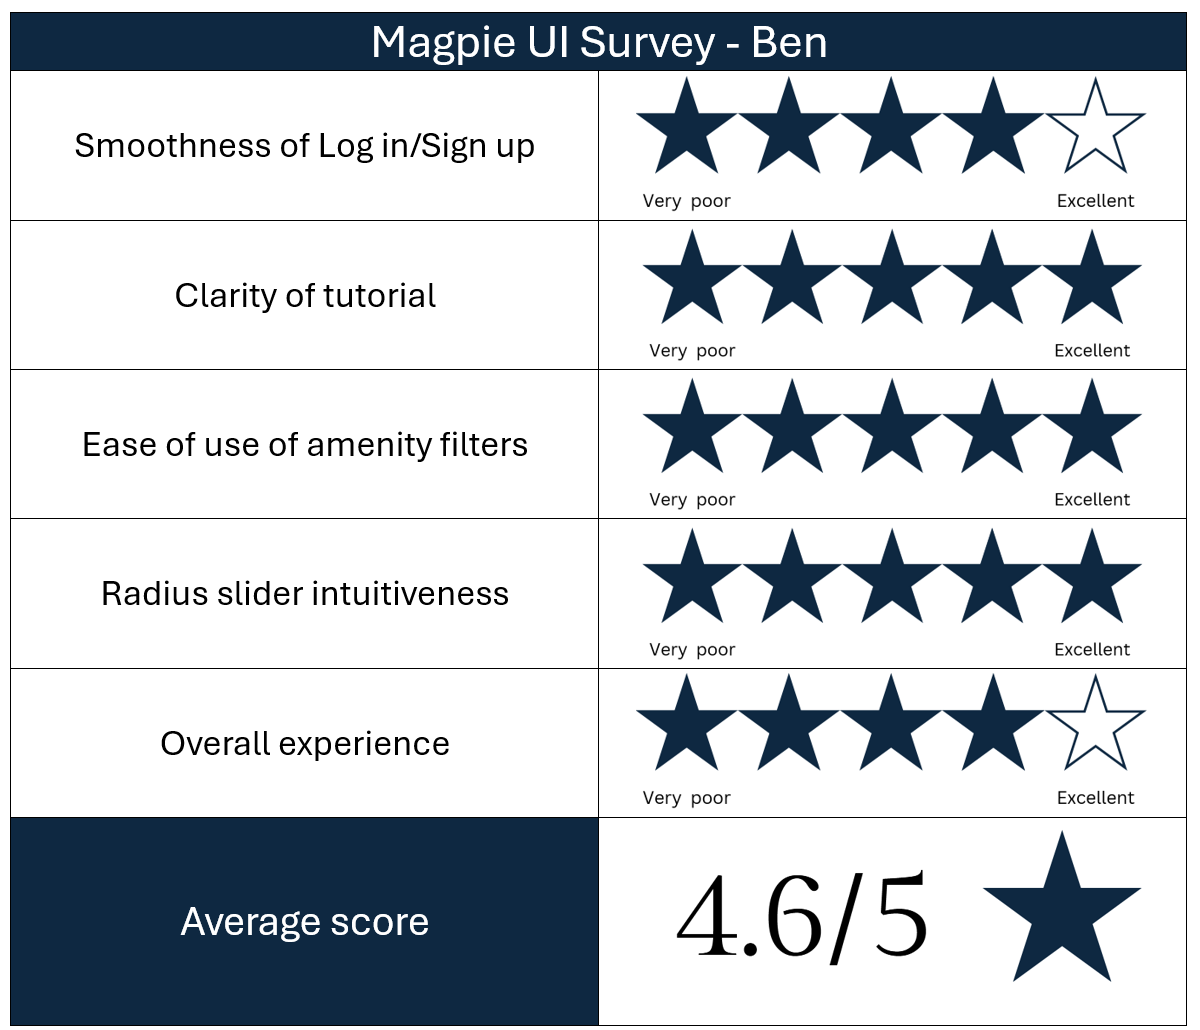
\includegraphics[width=0.8\textwidth]{images/survey-ben.png}
    \caption{User Evaluation - UI Score Ben}
\end{figure}

\newpage
\subsubsection{User 6 - Jakub}
Jakub is a professional with a construction and technological background. They were recruited towards the end of product development to test Magpie. They are considered a casual user.\\\\
This was an uncontrolled test session where Jakub discovered the application on their own, discussing each feature, testing each feature, and were then given a small scenario "Put yourself in the shoes of an urban planner..." to obtain a different kind of feedback from previous sessions.\\\\
%table of Jakub's general tasks
\begin{table}[h!]
    \centering
    \caption{Usability testing Tasks - Jakub}
    \begin{tabular}{|p{0.4\textwidth}|p{0.1\textwidth}|p{0.1\textwidth}|p{0.1\textwidth}|p{0.1\textwidth}|}
        \hline
        \textbf{Task}                 & \textbf{Status} & \textbf{Difficulty} & \textbf{Errors}    \\
        \hline
        Load Magpie application       & Complete        & 1                   & N/A                \\
        \hline
        Sign up                       & Complete        & 1                   & N/A                \\
        \hline
        Log in                        & Complete        & 1                   & N/A                \\
        \hline
        Complete tutorial             & Complete        & 1                   & N/A                \\
        \hline
        Place cursor on map           & Complete        & 1                   & N/A                \\
        \hline
        Zoom in and out               & Complete        & 1                   & N/A                \\
        \hline
        Hold map and navigate         & Complete        & 1                   & N/A                \\
        \hline
        Adjust radius big/small       & Complete        & 1                   & N/A                \\
        \hline
        Clear marker \& radius        & Pass            & 3                   & Did not see button \\
        \hline
        Deselect all amenities        & Complete        & 1                   & N/A                \\
        \hline
        Select one or more amenities  & Complete        & 1                   & N/A                \\
        \hline
        Find tutorial and exit midway & Skipped         & Skipped             & Skipped            \\
        \hline
        Log out                       & Complete        & 1                   & N/A                \\
        \hline
    \end{tabular}
\end{table}
\textbf{Main takeaways from Jakub's session: }this tool simplifies the search for amenities however there are certain items that need to be considered to improve the application:
\begin{itemize}
    \item \textbf{Log in/Sign up: }Email verification should be included, so that the user can confirm they have successfully signed up and also for security purposes.
    \item \textbf{Map: }some of the amenity data doesn't have accurate locations, for example public toilets seem to be off by longitude, and multi-storey parking data seems incomplete. Also, water fountains are very hard to find on the map, we should consider changing its colour. Same with the profile and tutorial icon, they are hard to spot on the map. They would also like to double click on the map to clear it, more intuitive for them. And last thing, amenities with small count are hard to find in the radius, maybe make them more visible somehow.
    \item \textbf{History feature: }doesn't see the use for a casual user, and again same for this tool, doesn't see the use for them as a casual user but could be useful for a target user.
    \item \textbf{Extra features: }Search functionality would be very useful for those that are lookin for a spot but don't know where it is located visually. Also, an export feature would be useful for the scenario of urban planning, if I'm to put a report together, a visual from this tool would be helpful for illustration.
\end{itemize}
A notable behaviour indicator from them was that they tried to interact with the elements during onboarding, as have previous users. Due to technical limitations, we have been unable to make that happen. Future work.\\\\
Overall, the tooltips for the icons is very interesting, a suggestion would be to add the type of parking to car parking and the zoning information as well as tariff.
\textbf{Score from survey: }
%jakub survey score
\begin{figure}
    \centering
    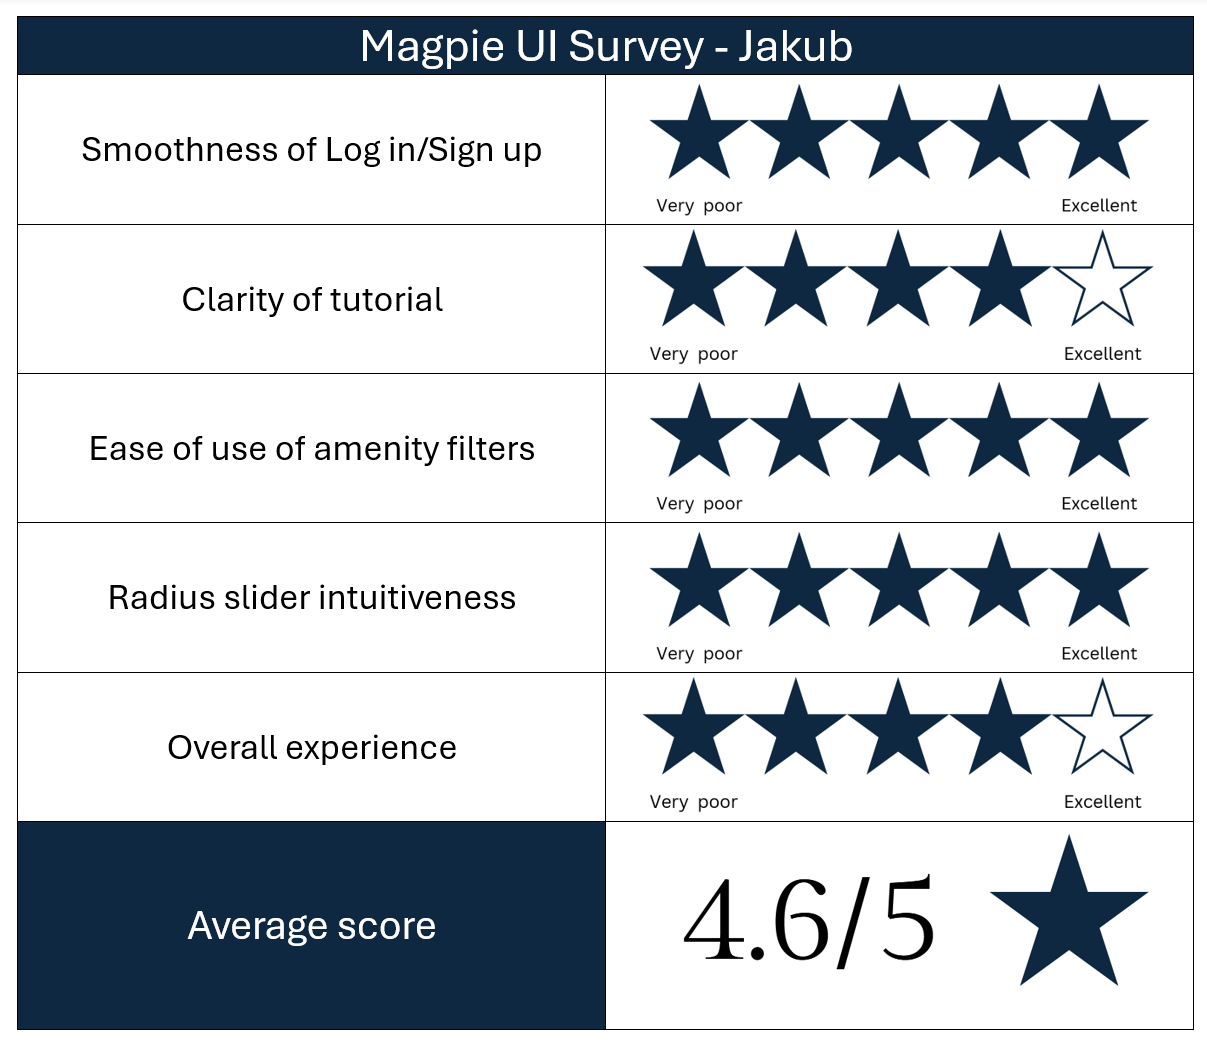
\includegraphics[width=0.8\textwidth]{images/survey-jakub.png}
    \caption{User Evaluation - UI Score Jakub}
\end{figure}

\newpage
\subsubsection{User 7 - Bryan Boyle}
Professional user Bryan

\newpage
\subsubsection{User 8 - Anonymous}
Professional user Sarah

\newpage
\subsubsection{User 9 - Anonymous}
Professional user Odran
